\documentclass[oneside,10pt]{book}


\usepackage{cdtBook}
\usepackage{usecases}
\usepackage{gensymb}

\begin{document}

\subsection{IU1 Página principal}

\subsubsection{Objetivo}
Mostrar información general a los usuarios y dar acceso a las funciones del sistema.

\subsubsection{Diseño}
Esta pantalla aparece al ingresar al sitio desde la URL pizza.escom.xyz.

\begin{figure}[htbp!]
	\centering
	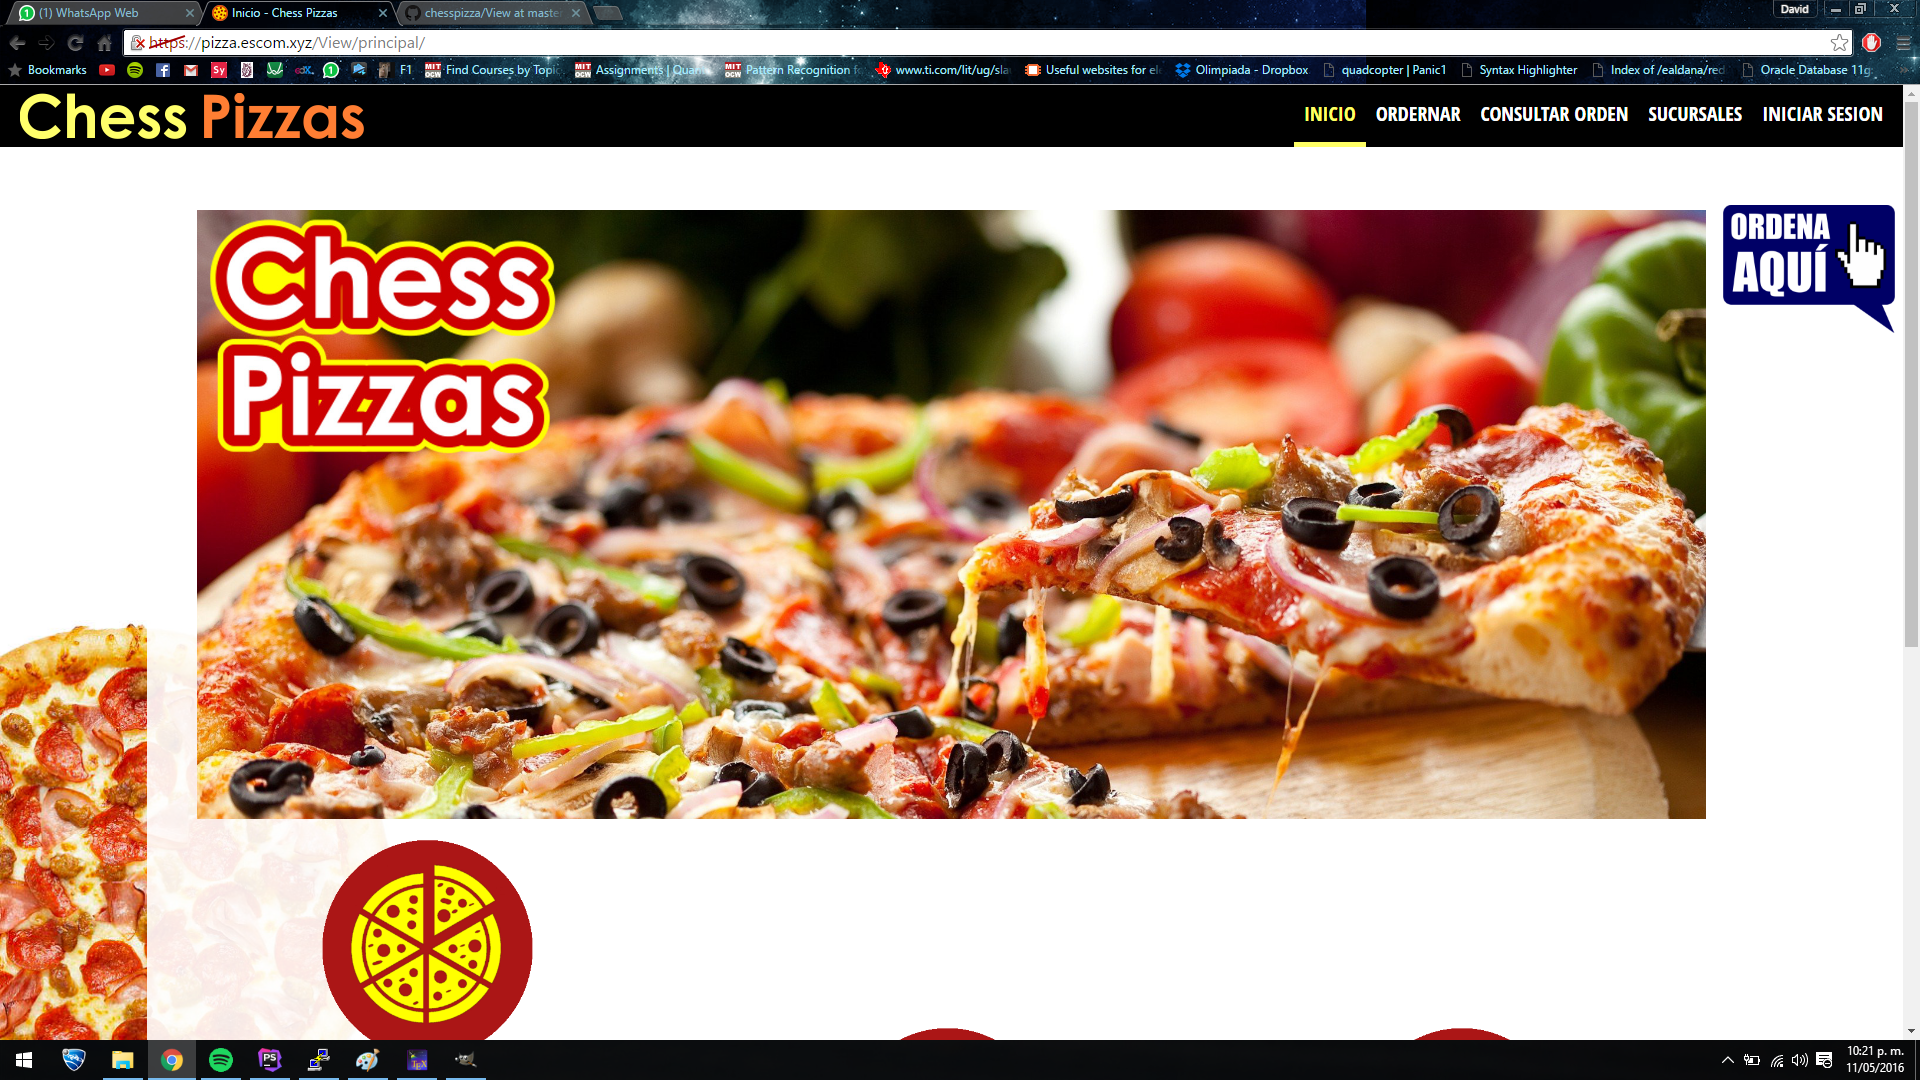
\includegraphics[width=1\textwidth]{img/principal}
	\caption{IU1 Página principal}
\end{figure}


\subsubsection{Salidas}
\begin{itemize} 
	\item Imágenes representativas de la cadena
	\item Menú de navegación
\end{itemize}
\subsubsection{Entradas}
\begin{itemize}
	\item Ninguna
\end{itemize}

\subsubsection{Comandos}
\begin{itemize}
	\item \IUbutton{INICIO}:  Muestra la interfaz \IUref{UI1}{Página principal}.	
	\item \IUbutton{ORDENAR}:  Muestra la interfaz \IUref{UI3}{Ordenar pizza}.	
	\item \IUbutton{CONSULTAR ORDEN}:  Muestra la interfaz \IUref{UI4}{Consultar orden(cliente)}.	
	\item \IUbutton{SUCURSALES}:  Muestra la interfaz \IUref{UI}{}.	
	\item \IUbutton{INICIAR SESIÓN}:  Muestra la interfaz \IUref{UI2}{Iniciar sesión}.	
\end{itemize}

\subsubsection{Mensajes}
Ninguno

\subsection{IU8 Consultar órdenes(chef)}

\subsubsection{Objetivo}
Que los chefs obtengan la información de las órdenes que deben preparar

\subsubsection{Diseño}
Esta pantalla aparece al iniciar sesión como chef en el sistema.

\begin{figure}[htbp!]
	\centering
	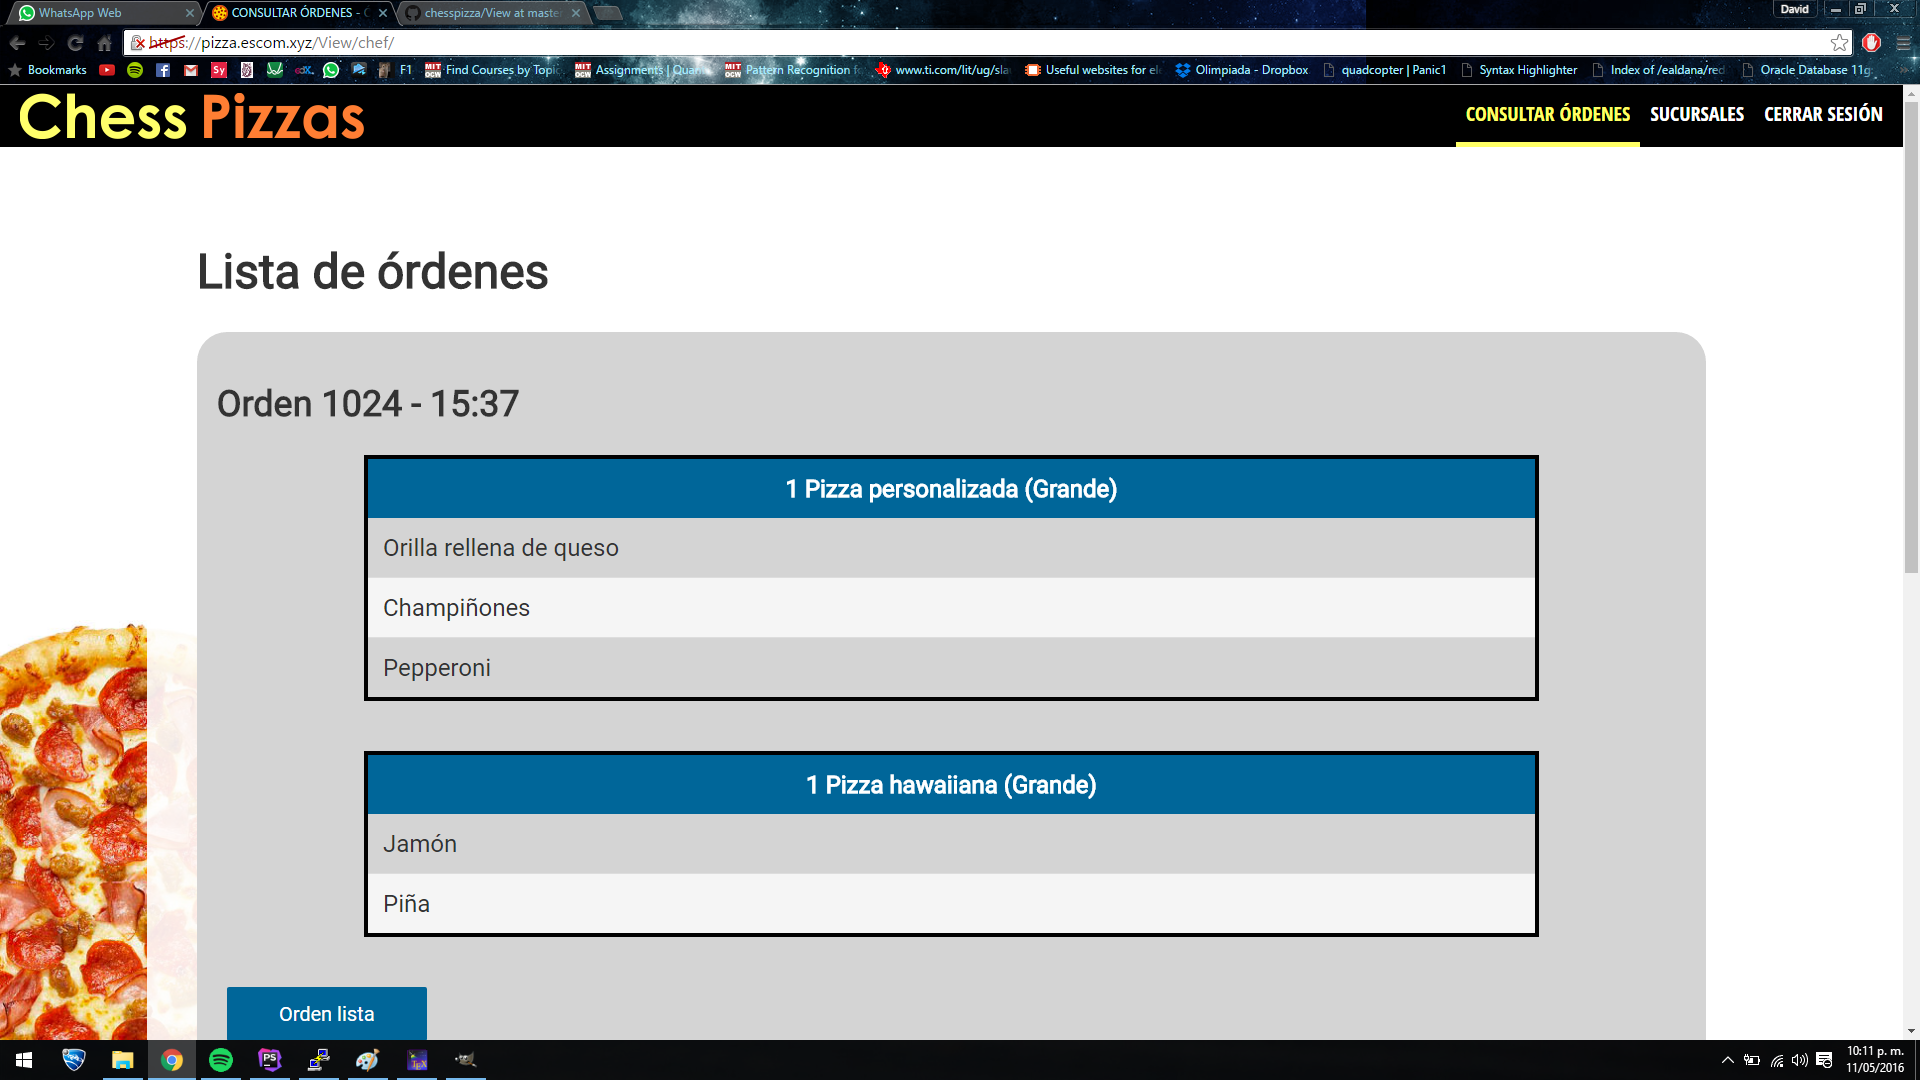
\includegraphics[width=1\textwidth]{img/chef}
	\caption{IU8 Consultar órdenes(chef)}
\end{figure}


\subsubsection{Salidas}
\begin{itemize} 
	\item Lista de órdenes de la sucursal a la que pertenece el chef, ordenadas primero la más reciente, con la siguiente información:
	\begin{itemize}
		\item Número de orden
		\item Hora de orden
		\item información de cada pizza de la orden:
		\begin{itemize}
			\item Cantidad
			\item Nombre de pizza en caso de ser especial o en otro caso se le asigna el nombre "Pizza personalizada"
			\item Lista de ingredientes
		\end{itemize}
	\end{itemize}
	\item Nota: La lista se actualizará cada 15 segundos
\end{itemize}
\subsubsection{Entradas}
\begin{itemize}
	\item Identificador de sucursal
\end{itemize}

\subsubsection{Comandos}
\begin{itemize}
	\item \IUbutton{Orden lista}:  Se hace click en el botón cuando una orden ha sido preparada en su totalidad y está lista para ser repartida. Al hacer click sobre él, el estádo de la orden se modifica y es removida de la lista de ordenes por preparar.
\end{itemize}

\subsection{IU2 Iniciar Sesión}

\subsubsection{Objetivo}
Controlar el acceso a ciertas partes del sistema, de manera que solo personas autorizadas puedan utilizar las funcionalidades protegidas.


\subsubsection{Diseño}
Esta pantalla aparece al presionar la opción ``Iniciar sesión'' desde la pantalla principal


\begin{figure}[htbp!]
	\centering
	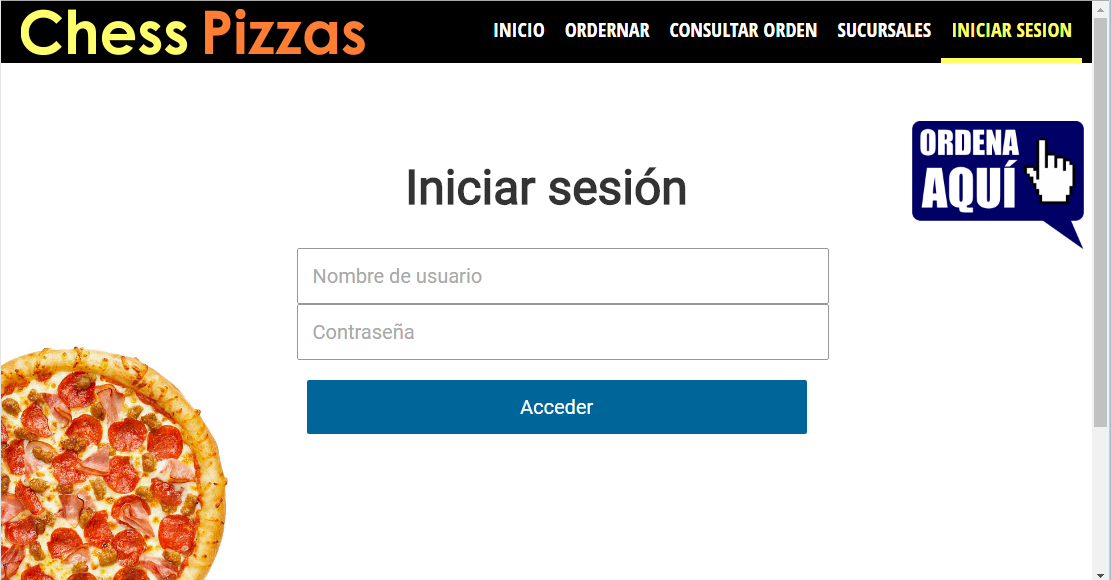
\includegraphics[width=1\textwidth]{img/iniciar_sesion}
	\caption{IU8 Consultar órdenes(chef)}
\end{figure}

\begin{figure}[htbp!]
	\centering
	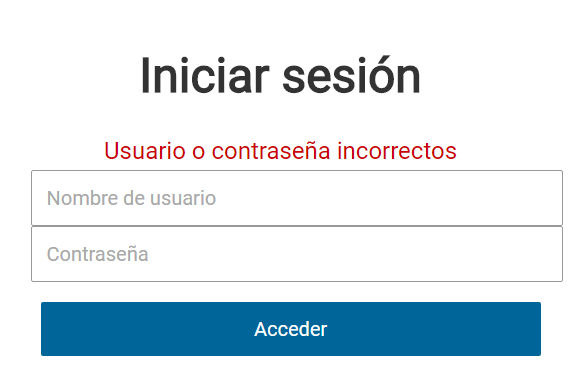
\includegraphics[width=1\textwidth]{img/iniciar_sesion2a}
	\caption{IU8 Consultar órdenes(chef)}
\end{figure}

\begin{figure}[htbp!]
	\centering
	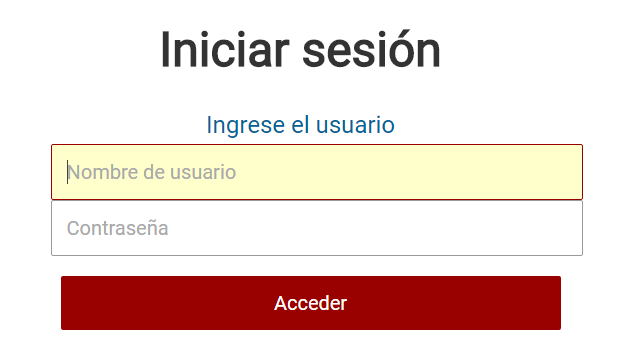
\includegraphics[width=1\textwidth]{img/iniciar_sesion2b}
	\caption{IU8 Consultar órdenes(chef)}
\end{figure}

\begin{figure}[htbp!]
	\centering
	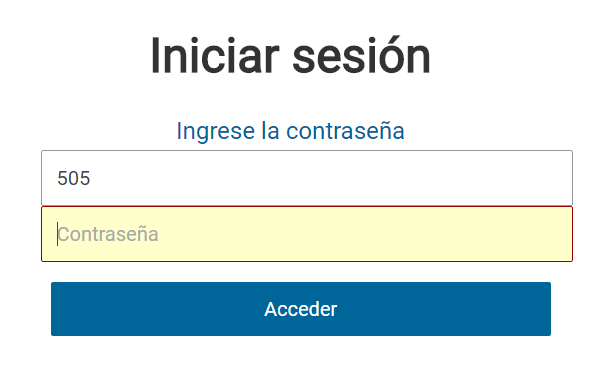
\includegraphics[width=1\textwidth]{img/iniciar_sesion2c}
	\caption{IU8 Consultar órdenes(chef)}
\end{figure}


\subsubsection{Salidas}
\begin{itemize} 
	\item Lista de órdenes de la sucursal a la que pertenece el chef, ordenadas primero la más reciente, con la siguiente información:
	\begin{itemize}
		\item Número de orden
		\item Hora de orden
		\item información de cada pizza de la orden:
		\begin{itemize}
			\item Cantidad
			\item Nombre de pizza en caso de ser especial o en otro caso se le asigna el nombre "Pizza personalizada"
			\item Lista de ingredientes
		\end{itemize}
	\end{itemize}
	\item Nota: La lista se actualizará cada 15 segundos
\end{itemize}
\subsubsection{Entradas}
\begin{itemize}
	\item Nombre de usuario: Cadena de números que representan el código de la sucursal. 
	\item Contraseña: Cadena de caractéres no mayor a 30.
\end{itemize}

\subsubsection{Mensajes}
\begin{itemize}
	\item {\bf MSG2a} ``Usuario o contraseña incorrectos''.
	\item {\bf MSG2b} ``Ingrese el usuario''.
	\item {\bf MSG2c} ``Ingrese la contraseña''.
\end{itemize}

\subsubsection{Comandos}
\begin{itemize}
	\item \IUbutton{Acceder} Al presionarse el sistema verifica que se haya ingresado el campo ``Nombre de usuario'', de lo contrario muestra MSG2b. Posteriormente verifica que se haya ingresado el campo contraseña, de lo contrario se muestra MSG2c. Además el sistema consulta con la base de datos que exista el código de la sucursal y que la contraseña ingresada coincida con la contraseña registrada. Si el código y la contraseña coinciden muestra la pantalla principal de control de la sucursal, de lo contrario muestra MSG2a.
\end{itemize}


\end{document}


